\section{Experiments \& Results}
\label{sec:experiments}
\begin{figure}
	\begin{center}
		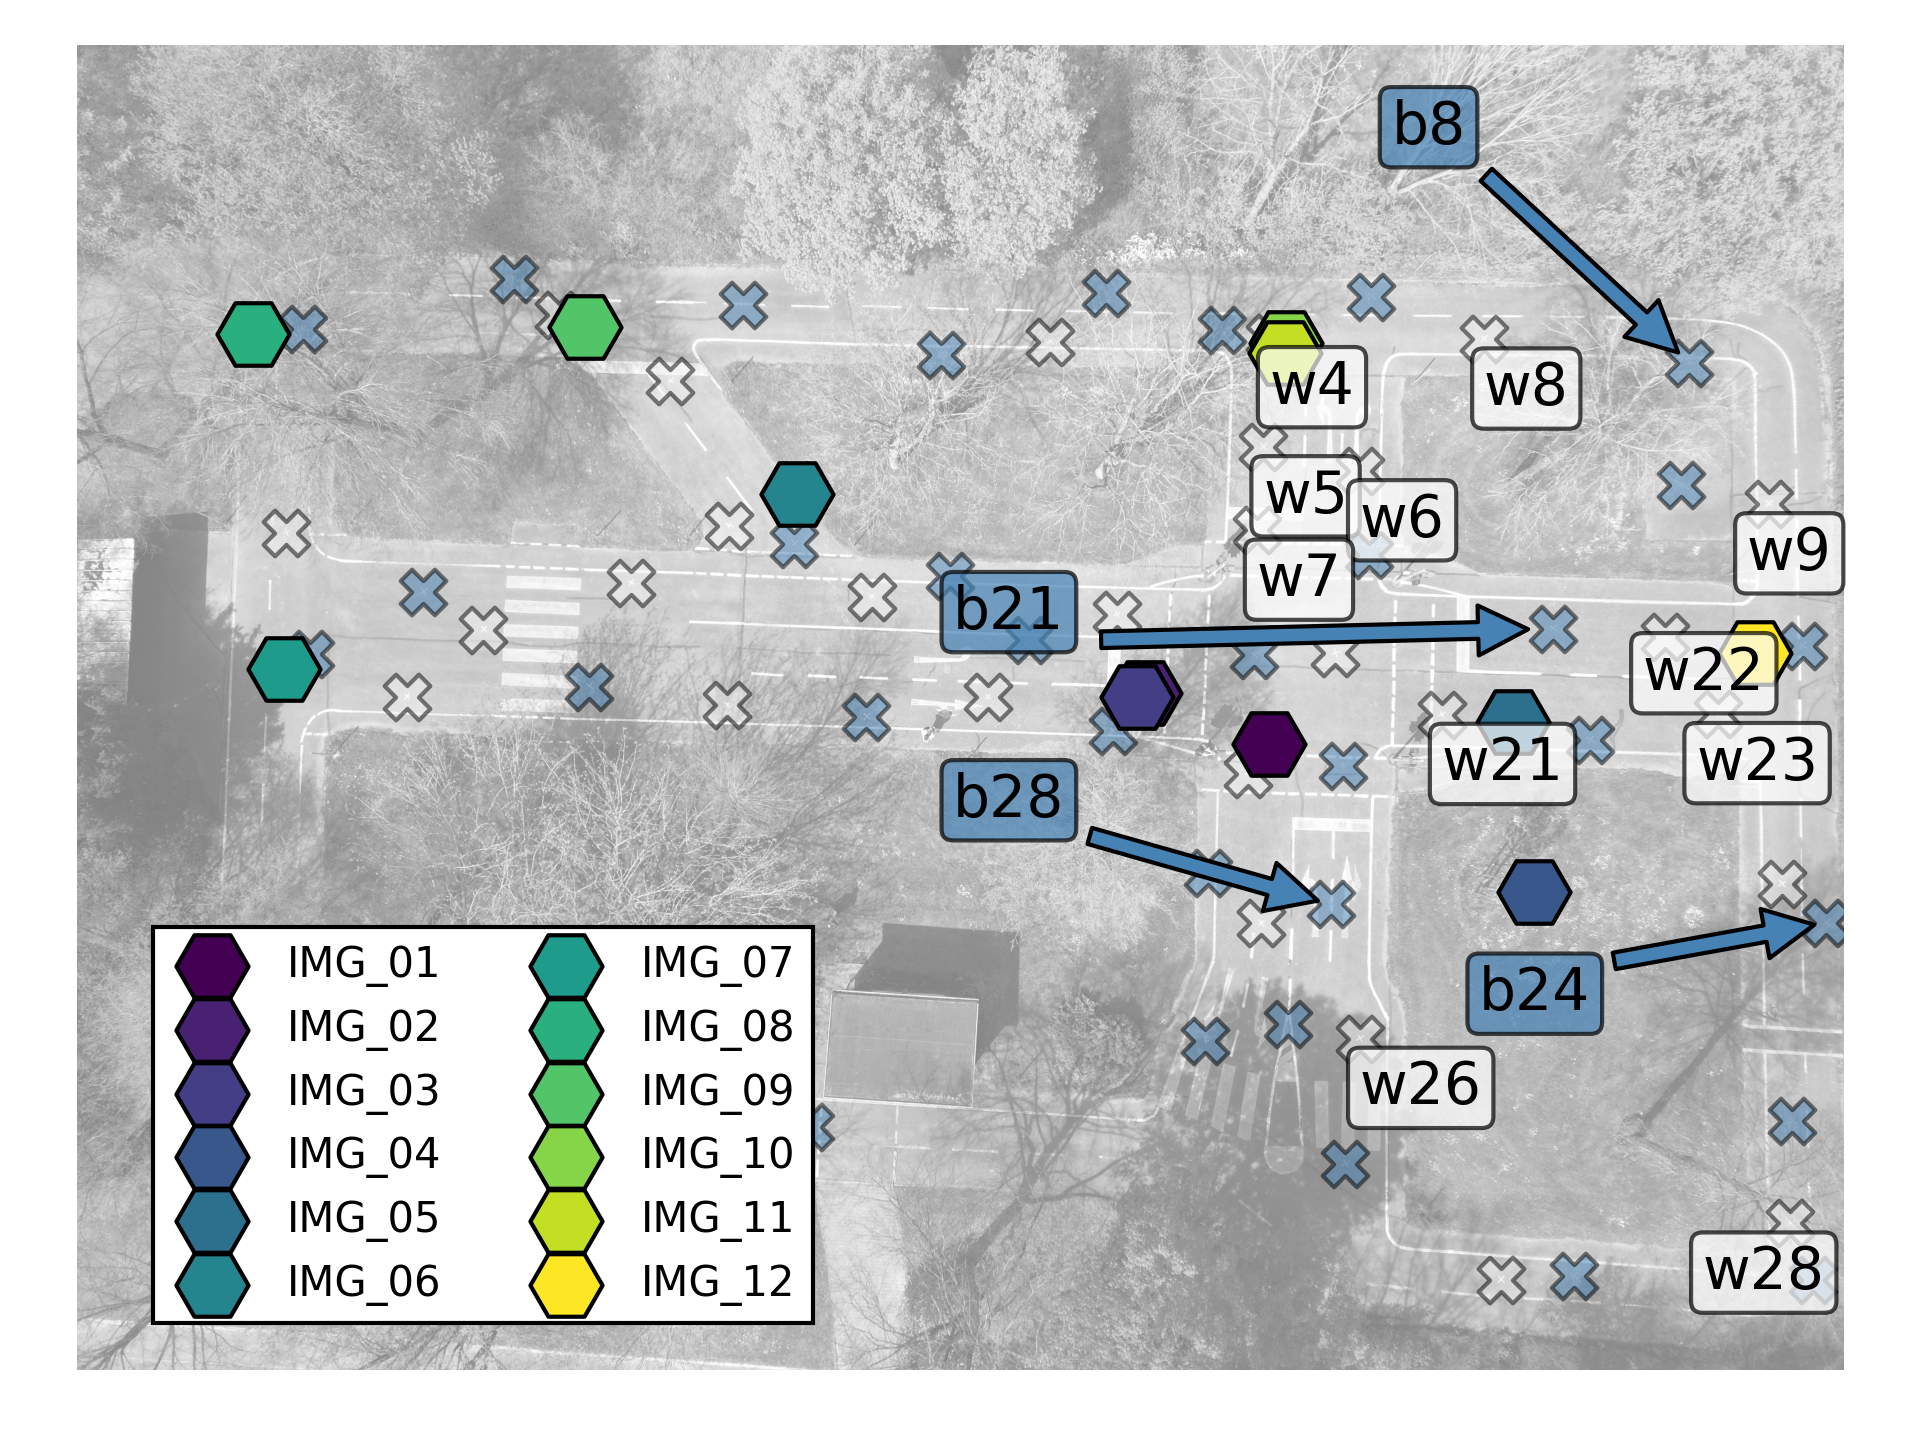
\includegraphics[width=0.45\textwidth]{figures/camera_positions.png}
	\end{center}
	\caption{The top view with the reference (white crosses) and validation points 
	(blue crosses), and the estimated $x,y$-positions for each camera (hexagons) within 
	the shared coordinate system.}
	\label{fig:positions}
\end{figure}

To evaluate the accuracy of the ESCal method, we tested the homography within 
a large-scale, non-planar environment of about $66$ m $\times$ $42$ m.
We marked a traffic-practice area with 62 points by physically taping crosses 
on the ground, distinguishing between 28 reference points and 34 validation points. 
The reference points are used to determine the homography matrices, 
while the validation points are used to calculate the reprojection errors. 
The dataset is publicly available on GitHub\footnote{https://github.com/Sntz91/ESCal}. 

Specifically, we captured the top view image using a DJI Mini 3 Pro consumer drone, 
covering the scene from a bird's-eye view with a pitch of $-90$ degrees at 
$50.2$ m height. Furthermore, we captured 12 
perspective view images from various angles and heights, each featuring 
different reference and validation point combinations\textemdash with varying 
quality. The Inertial Measurement Unit (IMU) of our drone logged the pitch 
and height for every image. The camera's sensor produces 12 MP images of 
size $4000\times3000$ px. The twelve produced images IMG\_01, ..., IMG\_12 
simultaneously represent the twelve camera positions as seen in Figure 
\ref{fig:positions}.

\subsection{Finding the Camera's Pose}
As stated in Section \ref{sec:solution}, we determined the camera's 
intrinsics in advance using Zhang's \cite{zhang2000} method. Moreover, 
the dataset contains at least four marked point correspondences between each 
perspective view and the top view. Accordingly, we determined the 
homography matrix $\mathrm{H}_p$ for every camera. Consequently, we can 
calculate every camera's location and rotation using Equation 
(\ref{eq:pose_background}).
Table \ref{tab:camera_pose} compares the logged results with our predictions.

\begin{table}[hb]
	\caption{Accuracy of the estimated camera poses}
		\begin{tabular*}{\columnwidth}{@{\extracolsep{\fill}} l cccc}
			\toprule
			&
			\multicolumn{2}{l}{\textbf{Estimated by ESCal}} & 
			\multicolumn{2}{l}{\textbf{Measured by UAV}} \\
			& Height [m] & Pitch [deg] & Height [m] & Pitch [deg] \\
			\midrule
			IMG\_01 & 10.0 & -40.5 & 10.3 & -43.0 \\
			IMG\_02 & 10.1 & -41.0 & 10.3 & -43.0 \\
			IMG\_03 & 10.2 & -41.7 & 10.3 & -43.0 \\
			IMG\_04 & 10.3 & -41.8 & 10.4 & -43.0 \\
			IMG\_05 & 10.0 & -36.4 & 10.3 & -38.1 \\
			IMG\_06 & 2.6  & -24.7 & 3.2  & -27.8 \\
			IMG\_07 & 10.3 & -34.9 & 10.3 & -38.5 \\
			IMG\_08 & 2.8  & -29.9 & 2.8  & -32.1 \\
			IMG\_09 & 9.8  & -41.0 & 10.1 & -43.5 \\
			IMG\_10 & 7.7  & -36.2 & 7.9  & -38.7 \\
			IMG\_11 & 7.7  & -44.4 & 7.9  & -47.3 \\
			IMG\_12 & 10.3 & -34.7 & 10.3 & -36.8 \\
			\bottomrule
		\end{tabular*}
	\label{tab:camera_pose}
\end{table}

This leads to an average rotational error of $2.4$ degrees. However, 
several measurement errors contribute to this result. For example, the ground 
truth values from the drone's logs contain inherent measurement inaccuracies. 
Additionally, wind affects the drone's pose, violating our assumption of an 
exact $-90$-degree pitch in our top view. In fact, we observe a 
systematic error of approximately $+2$ degrees. 
Figure \ref{fig:positions} shows 
the estimated positions for the twelve cameras within the top view.


\subsection{Effective Field of View}

To determine a camera’s field of view, we specify the ground plane within 
an image and adjust the polygon to discard occluded areas. 
We obtain the camera's effective field of view by transforming the vertices
into the shared top view (Figure \ref{fig:fov}). Repeating this process 
for each camera allows to map the collective coverage of the CN.

\begin{figure}[t]
	\centering
	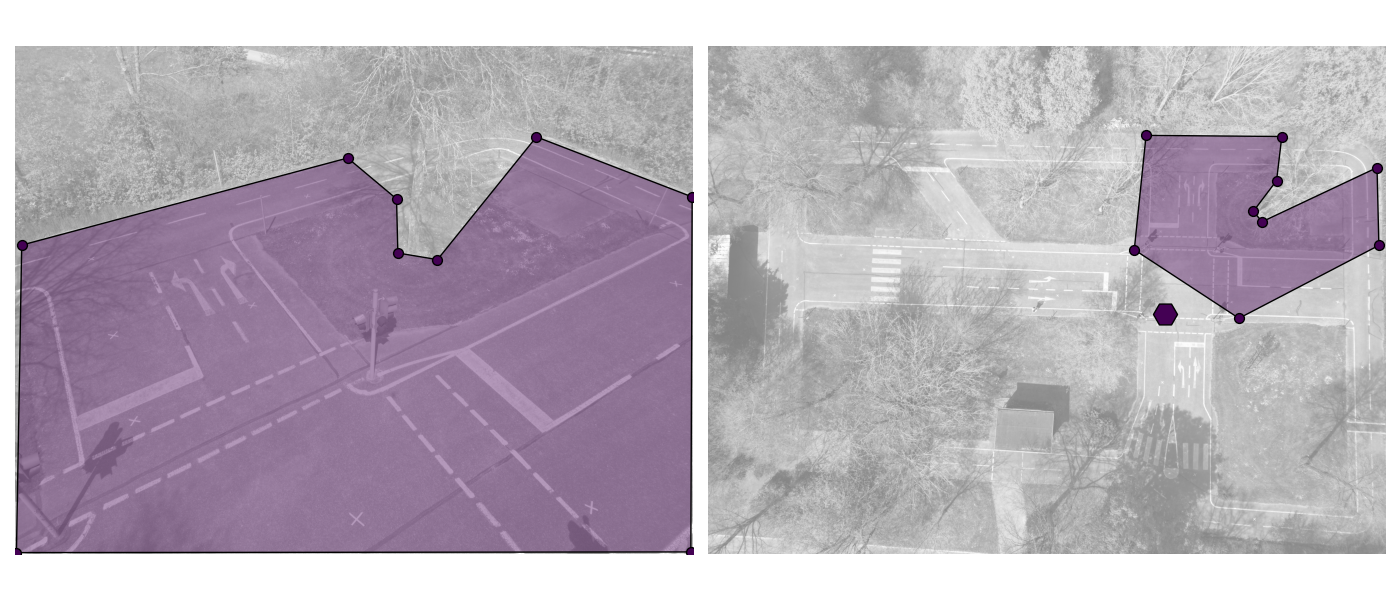
\includegraphics[width=0.45\textwidth]{figures/predicted_fov.png}
	\caption{Example for one camera (IMG\_01): Transforming an effective field 
	of view into the top view. The hexagon shows the camera's position.}
	\label{fig:fov}
\end{figure}


\subsection{Overall Accuracy of a Homography within Real-World Scenarios}
We consider all captured validation points to estimate the error 
$\mathrm{E}_p$ (in pixels) for each perspective view. We transform 
each validation point from the perspective view to the top view, 
and calculate the distance to its actual location accordingly:
\begin{equation}
\begin{aligned}
\mathrm{E}_{p} = \frac{1}{n_\text{val}} \sum_{i=1}^{n_\text{val}}{d(\mathbf{X}_{t}^{i}, \mathrm{H}_p\mathbf{x}_{p}^i)},
\end{aligned}
\end{equation}
where the function $d$ returns the Euclidean distance; $n_\text{val}$ is the number of 
validation points; $\mathbf{X}^{i}_{t}$ 
is the $i$-th validation point represented in world coordinates and serving as
ground truth; $\mathrm{H}_p$ is the corresponding homography matrix between 
the top-view and the $p$-th ($p \in \{ 1, ..., 12 \}$) perspective view; 
and $\mathbf{x}_{p}^i$ the corresponding validation point of the 
perspective view. 

Additionally, to calculate the error in meters rather than pixels, we need 
to define a scale factor, i.e., the number of pixels per meter within 
the top view\textemdash in 
our case, $54.67$ pixels per meter. Although this introduces a perspective error 
(as we used an entocentric lens), we captured the top view at $50.2$ meters height 
and can neglect it. 

Our findings, summarized in Table \ref{tab:results_overall}, provide a 
comprehensive overview of the experimental results. On average, our predicted 
points deviated from the ground truth by $15.28$ cm. However, it is 
noteworthy that this average includes various point compositions, 
image heights, and angles, leading to a wide range of results. 
The validation points within IMG\_03 only deviated by an average of 
$5.74$ cm (=$3.14$ px).

\begin{table}
\caption{Overall Results}
%\begin{tabular}{ |p{1.5cm}|p{1.5cm}|p{1.5cm}|p{1.5cm}|p{1.5cm}|p{1.5cm}|  }
% \begin{tabular}{|c | c c c c c|}
\begin{tabular*}{\columnwidth}{@{\extracolsep{\fill}} l ccccc}
\toprule
\textbf{Image} & \textbf{Err} & \textbf{Std} & \textbf{ValPts} &  \textbf{Angle} & \textbf{Alt} \\
& \textbf{[cm]} & \textbf{[cm]} & \textbf{[\#]} &  \textbf{[deg]} & \textbf{[m]} \\ [0.5ex]
\midrule
IMG\_01 & 6.95 & 3.40 & 6  & -43.0 & 10.3 \\
IMG\_02 & 6.93 & 2.62 & 11 & -43.0 & 10.3 \\
IMG\_03 & 5.74 & 5.67 & 9  & -43.0 & 10.3 \\
IMG\_04 & 9.74 & 8.03 & 18 & -43.0 & 10.4 \\
IMG\_05 & 7.67 & 6.74 & 14 & -38.1 & 10.3 \\
IMG\_06 & 65.13 & 59.83 & 3  & -27.8 & 3.2 \\
IMG\_07 & 11.90 & 9.09 & 18 & -38.5 & 10.3 \\
IMG\_08 & 34.03 & 25.38 & 12 & -32.1 & 2.8 \\
IMG\_09 & 8.94 & 4.15 & 10 & -43.5 & 10.1 \\
IMG\_10 & 10.19 & 8.96 & 13 & -38.7 & 7.9 \\
IMG\_11 & 7.59 & 6.04 & 6  & -47.3 & 7.9 \\
IMG\_12 & 8.53 & 5.48 & 18 & -36.8 & 10.3 \\
\bottomrule
\end{tabular*}
\label{tab:results_overall}
\end{table}

\subsection{Reference- and Validation Point Compositions}

\subsubsection{Number of Reference Points}
Basically, selecting four reference point pairs is enough to calculate a 
homography matrix $\mathrm{H}$. However, real-world measurements introduce 
noise. Accordingly, we can use optimization techniques and more point 
pairs to estimate $\mathrm{H}$, resulting in an overdetermined system of 
linear equations. By using more points, we can consider more scene 
characteristics. 

\begin{figure}
	\centering
		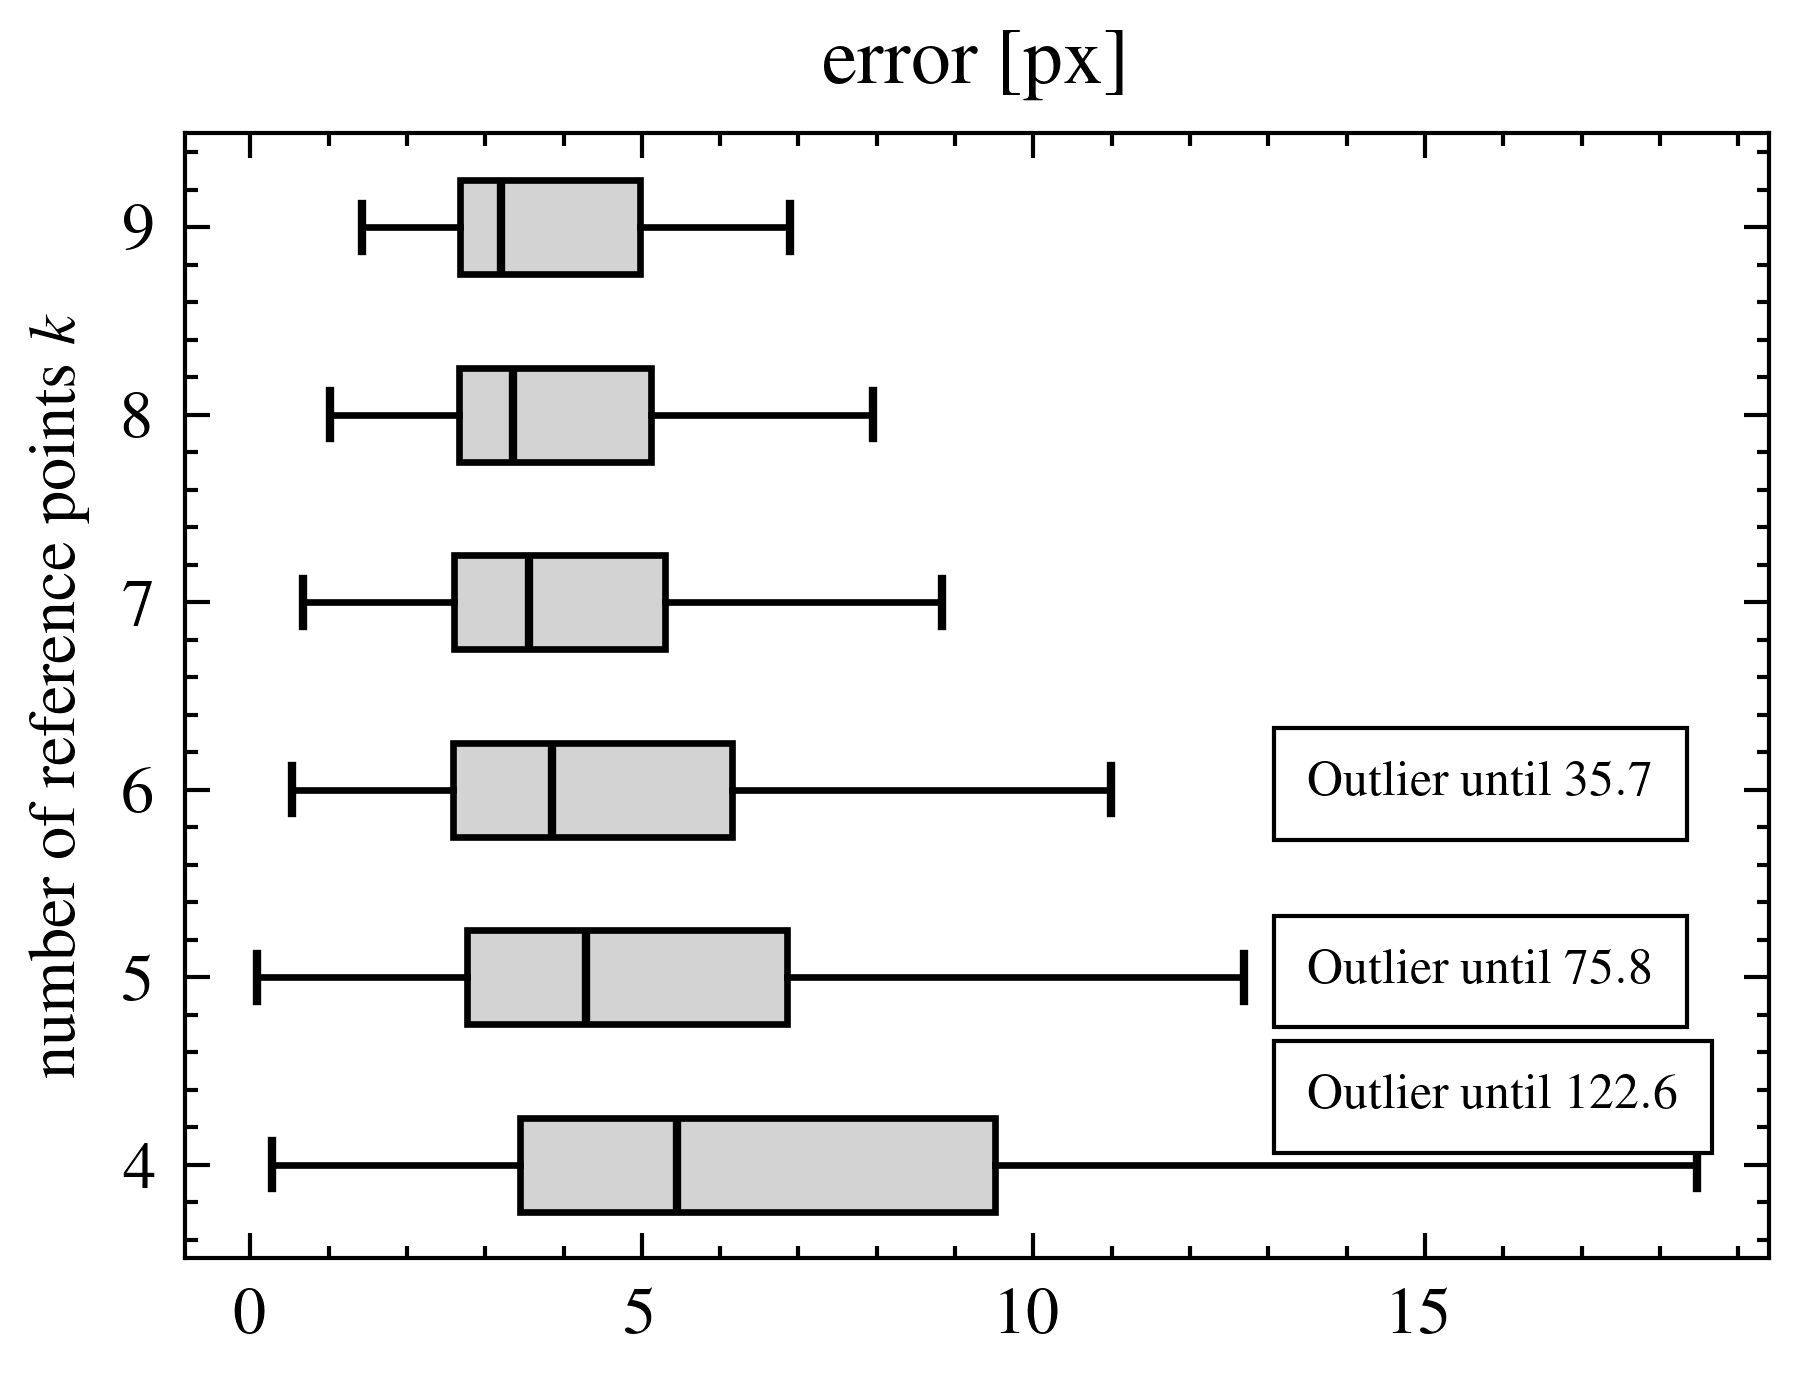
\includegraphics[width=0.45\textwidth]{figures/boxplot_errors_by_k_filtered.png}
	\caption{We chose all possible subsets of $k$ reference points and 
	calculated the error for each of the six validation points in IMG\_01 
	for each subset. Hence, we excluded all homographies with a 
	collinearity score of $< 1$.}
	\label{fig:boxplot_error_by_k_filtered}
\end{figure}

To determine the minimal number of points to be used, we analyze IMG\_01 
in more detail. The image contains nine reference points and six validation 
points, respectively. Previously, we used all reference points to calculate 
the corresponding homography matrix $\mathrm{H}_{01}$ and estimated the 
average error for all validation points, i.e., $6.95$ cm. 

In contrast to our earlier experiments, we use every possible composition 
of at least four reference points to determine $\mathrm{H}_{01}$ and estimate 
the average error. Hence, we conduct $382$ experiments for IMG\_01, 
consisting of the following point combinations, where $k$ denotes the number 
of used reference points to calculate $\mathrm{H}_{01}^i$, with 
$i \in \{ 1, 2, ..., 382 \}$:
\begin{align*}
	k=4 \rightarrow 126, k=5 \rightarrow 126, k=6 \rightarrow 84, \\
	k=7 \rightarrow 36, k=8 \rightarrow 9, k=9 \rightarrow 1.	
\end{align*}
Note that every single experiment calculates the errors for each 
validation point. Hence, the resulting dataset consists of $382 * 6 = 2.292$ 
data points.

Our random choice of reference points influences the homography matrix 
$\mathrm{H}_{01}^i$ and the quality of our reference, and validation points.
Using all nine reference points makes the homography less prone to 
degeneracy due to collinearity, validation points tend to be closer to 
reference points, etc. We will discuss those effects in detail subsequently. 
However, we exclude some point compositions with high collinearities
for our first, overall comparison to eliminate some significant outliers 
when only using four reference points.

Figure \ref{fig:boxplot_error_by_k_filtered} summarizes the results and implies that 
four reference points might be sufficient\textemdash but their composition is
crucial, even when neglecting collinearities.
With additional points, we may increase our confidence in obtaining
an accurate outcome. 


\subsubsection{Reference Point Compositions}
The choice of reference points enormously impacts a homography's quality. 
We have determined four factors for further investigation.

\paragraph{Collinearity}
To determine $\mathrm{H}_{01}$, we need at least four point pairs, i.e., 
we use $k=4$ reference points. However, the 
calculation collapses when at least three points are collinear. 
Nevertheless, collinearity rarely exists in 
real-world scenarios. Our experiments show that if three points are almost 
collinear, homographies still collapse. In the following, we will call those 
points collinear, even if, mathematically, they are not. 
IMG\_01 has three obvious collinear points: $w_4$, $w_5$, and $w_7$; 
calculating the homography with any other point produces degenerate 
solutions with intolerable errors. 

\begin{figure}
	\begin{center}
		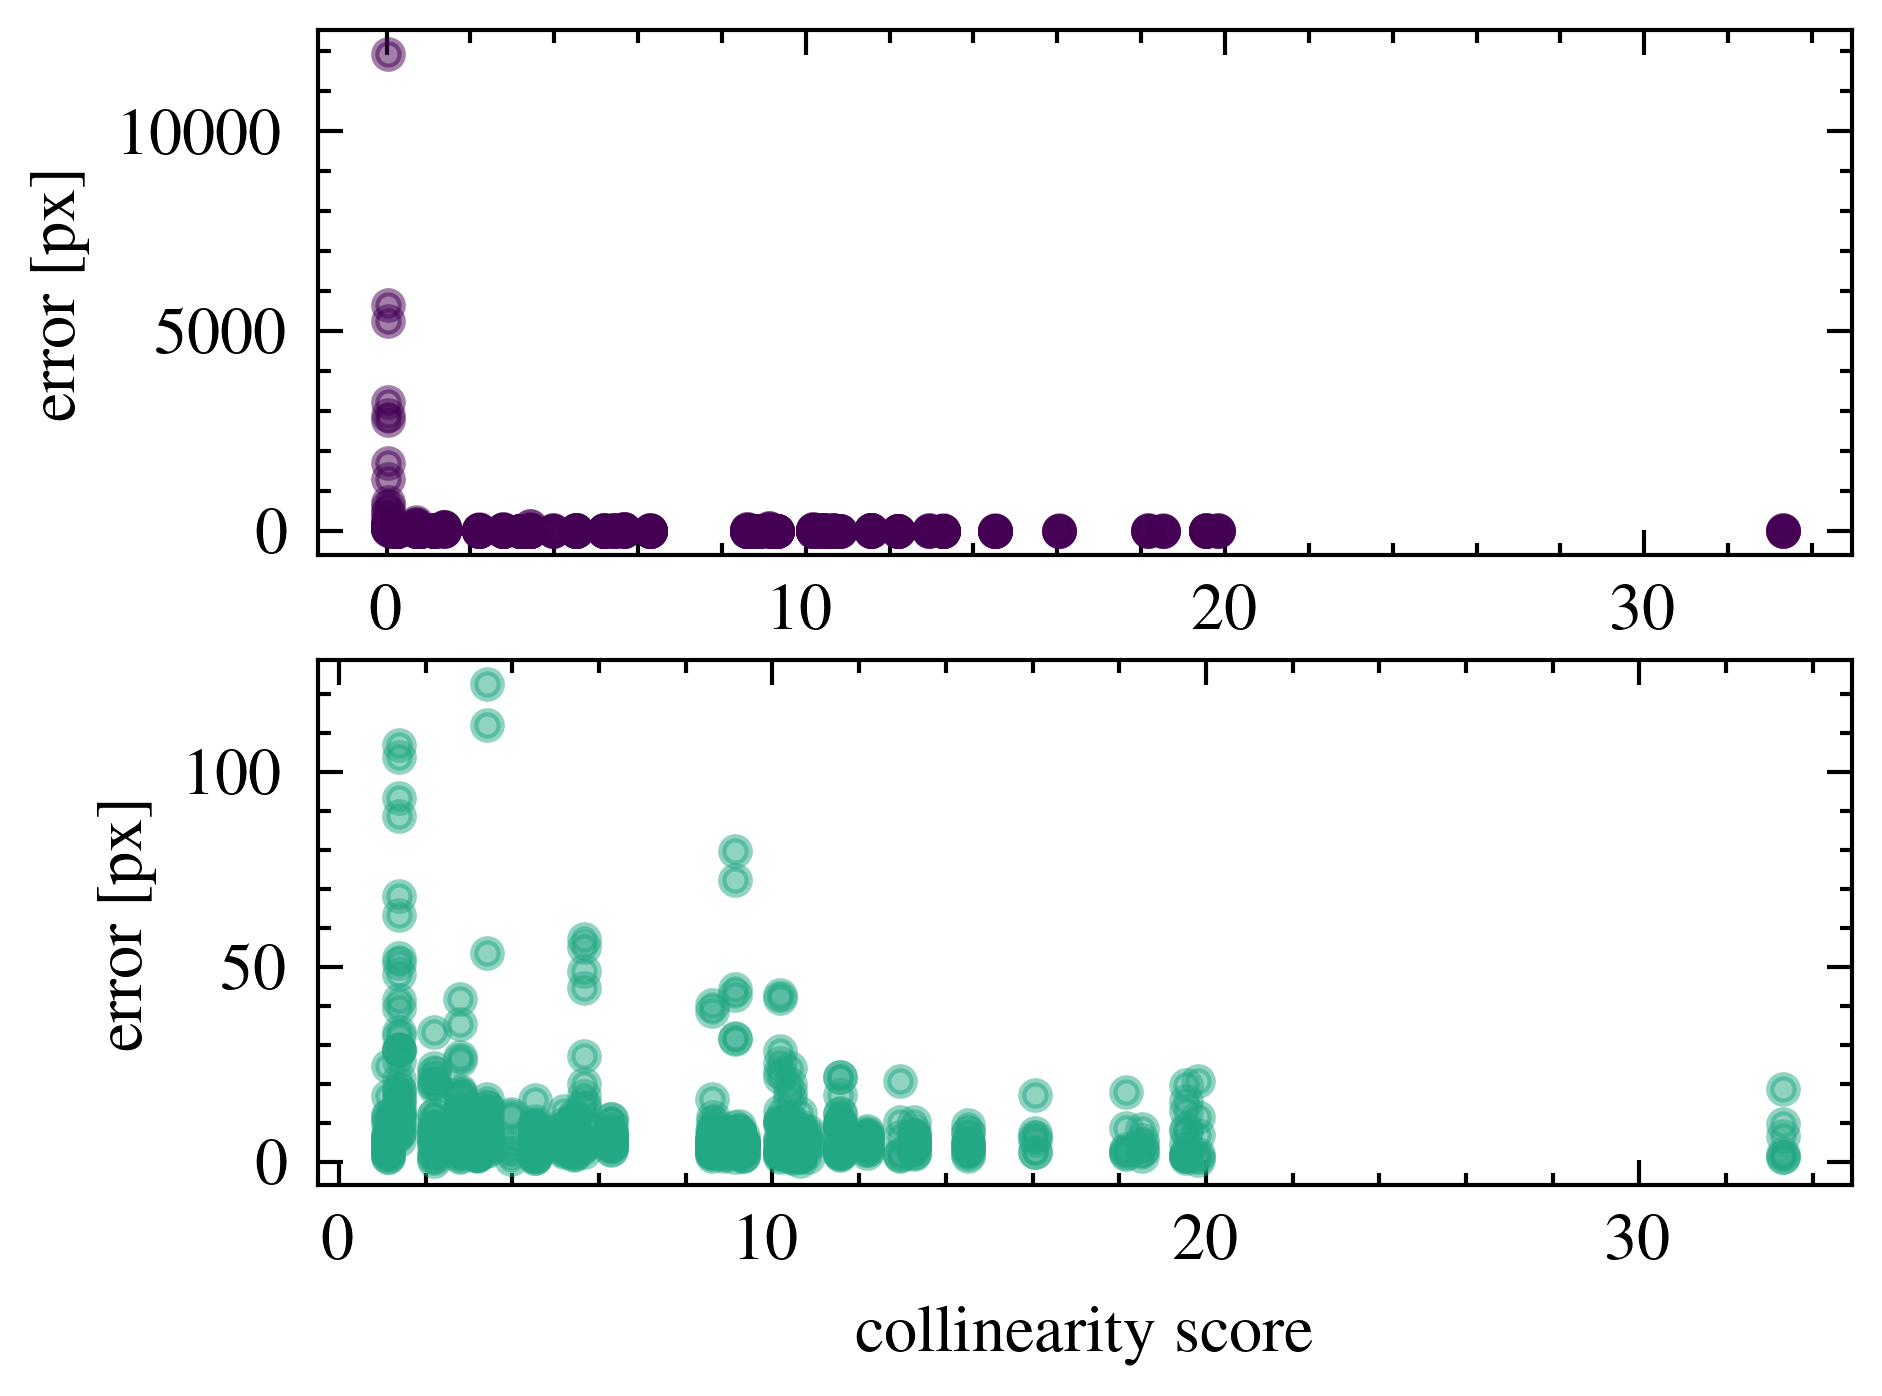
\includegraphics[width=0.45\textwidth]{figures/collinearity_error.png}
	\end{center}
	\caption{The error w.r.t. the collinearity scores (image above). The 
	error reduces significantly when excluding collinearity scores of 
	less than one (image below).}
	\label{fig:collinearity_error}
\end{figure}

However, $w_4$, $w_5$, and $w_7$ are not the only three collinear points. 
We propose to use the 
triangle inequality to determine collinearity. Given three reference points 
$w_i$, $w_j$, and $w_k$, and their corresponding edges $x$, $y$, and $z$, 
we calculate the collinearity $c(w_i, w_j, w_k)$ as follows:
\begin{equation}
\begin{aligned}
c(w_i, w_j, w_k) = \frac{x + y - z}{z},
\end{aligned}
\end{equation}
where $x,y,z\neq0$, $z > x$, and $z > y$. Because of the triangle inequality 
$z \geq x + y$. If three points lie within 
one line $c(w_i, w_j, w_k) = 0$. 
Note that a lower value corresponds to a higher collinearity.
For IMG\_01, this results in the collinearity values shown in 
Table \ref{tab:collinearity_values}.

\begin{table}[ht]
	\caption{Collinearity Scores for IMG\_01}\label{tab:collinearity_scores}
\begin{tabular*}{\columnwidth}{@{\extracolsep{\fill}} @{\hspace{40pt}}l r@{\hspace{40pt}}}
			\toprule
			\textbf{Reference Points} & 
			\textbf{Collinearity Value} \\
			\midrule
			w4, w5, w7 & 0.03 \\
			w5, w6, w9 & 0.12 \\
			w5, w6, w22 & 0.25 \\
			w4, w6, w21 & 0.69 \\
			w4, w8, w9 & 0.79 \\
			w4, w6, w22 & 1.12 \\
			... & ... \\
			w4, w6, w7 & 98.04 \\
			\bottomrule
		\end{tabular*}
	\label{tab:collinearity_values}
\end{table}

% \begin{figure}
	% \begin{center}
		% 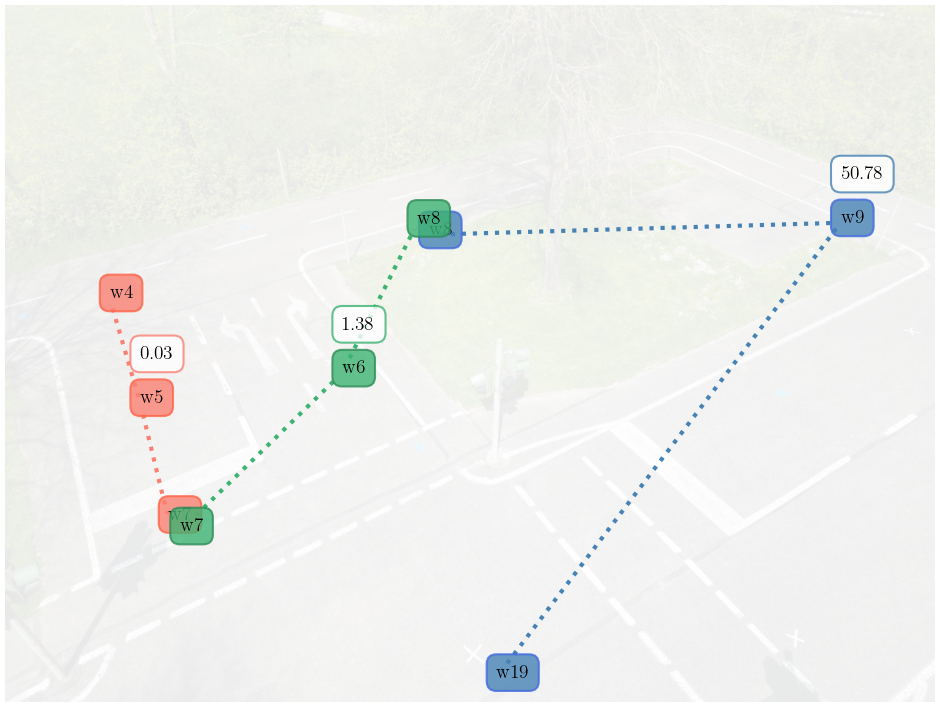
\includegraphics[width=0.35\textwidth]{figures/collinearity_examples.png}
	% \end{center}
	% \caption{This figure demonstrates three different collinearity values. 
		% When three reference points lie on the same line, the collinearity 
		% value approaches zero.}
		% \label{fig:collinearity_examples}
% \end{figure}

Each Homography $\mathrm{H}_{01}^i$, with $i \in \{ 1, 2, ..., 126 \}$ 
obtains $\begin{pmatrix} 4 \\ 3 \end{pmatrix} = 4$ collinearity values $c_1^i, c_2^i, c_3^i, c_4^i$.
If at least one subset is collinear, the homography collapses. 
Thus, we can take the smallest collinearity value to obtain the 
final collinearity score for $\mathrm{H}_{01}^i$:
\begin{equation}
\begin{aligned}
	c(\mathrm{H}_{01}^i) := \min{(c_1^i, c_2^i, c_3^i, c_4^i)}
\end{aligned}
\end{equation}

Thus, we can conduct the 126 experiments by selecting all reference point 
combinations within IMG\_01, where $k=4$. Every experiment produces 
six measurements. Figure \ref{fig:collinearity_error} shows the 
impact of collinearity. When excluding the twenty-nine homographies with a 
collinearity score of less than one, the error reduces drastically. 
We can improve a homography's robustness against collinearity by 
increasing the number of reference points $k$.

\paragraph{Distance to Next Reference Point}
The homography assumes that all points lie on the same plane ($Z=0$). The 
more we violate this assumption, the less precise our predictions are. 
Close points tend to have similar $Z$ coordinates generally. Suppose a 
validation point is close to a reference point: The $Z$ coordinate should be 
similar, and the error will be low, as we fitted the homography to 
this exact point.

However, suppose we used more than four points to calculate $\mathrm{H}$. 
Then, using optimization techniques, the argument loses some soundness. 
Nevertheless, the information is still being used and should be 
(on average) better than when no reference points are nearby.

\paragraph{Spanned Area}
Spanning larger areas entails considering more scene characteristics, 
correlating with the distance to the next reference points. 
Figure \ref{fig:error_by_area_and_distance} shows the impact of the 
spanned area and the validation point's distance to the next 
reference point, using the data from our collinearity experiments.
Large areas and close reference points decrease the 
errors by reducing the number of outliers.

\begin{figure}
	\begin{center}
		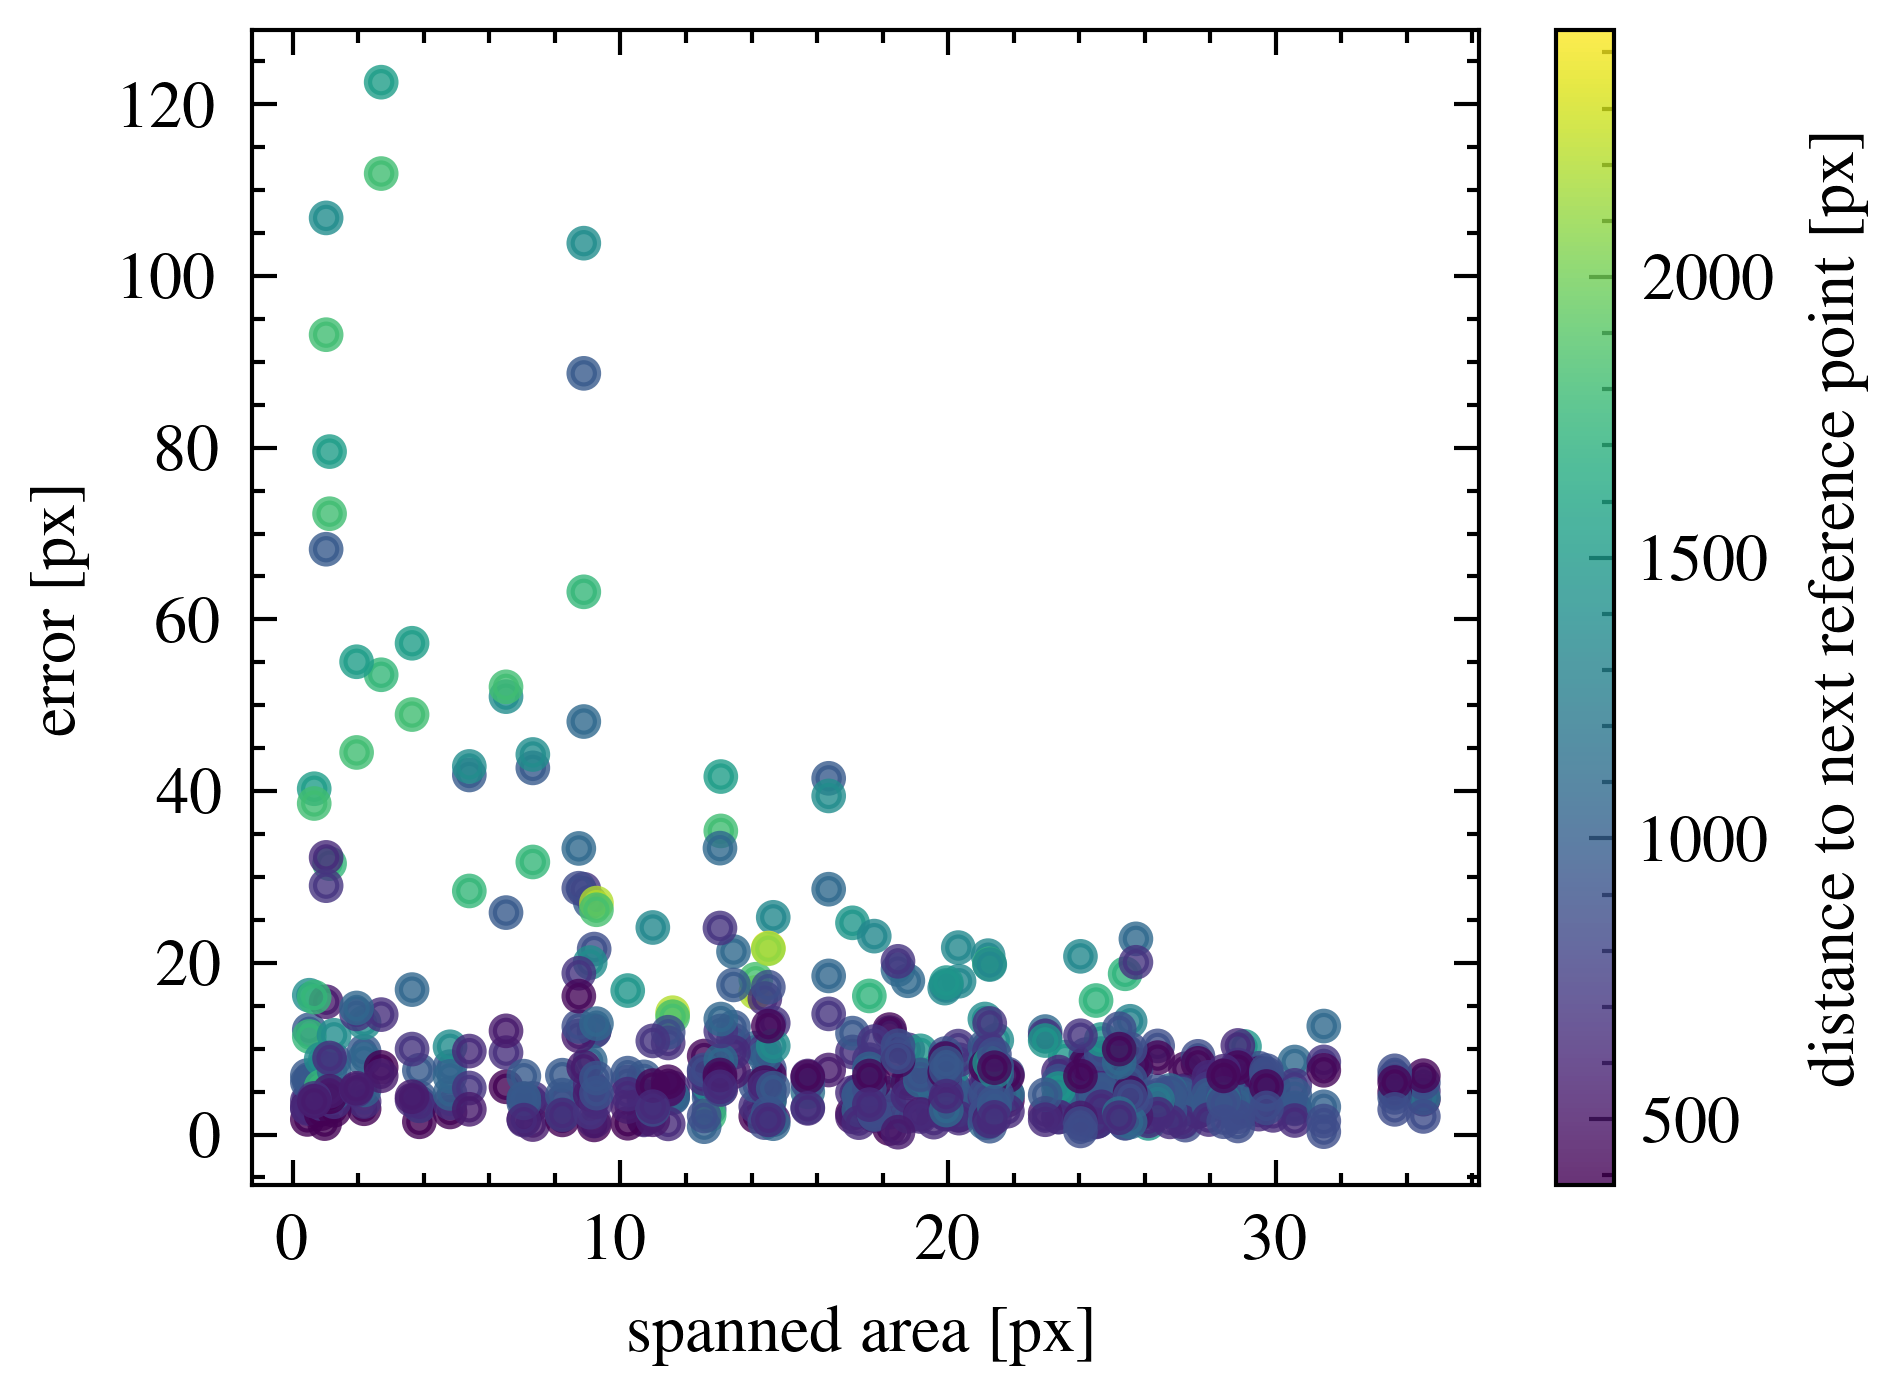
\includegraphics[width=0.45\textwidth]{figures/scatter_error_by_area_distance.png}
	\end{center}
	\caption{The error with respect to the spanned area and the distance
	to the next reference point, after excluding homographies with 
	a collinearity score of $c < 1$.}
	\label{fig:error_by_area_and_distance}
\end{figure}

\paragraph{Pixel Density}
The closer the validation point to the camera, the more pixels encircle it. 
A higher number of surrounding pixels results in a better prediction because 
the random noise within the perspective view loses its impact.

We propose to quantify a validation point's pixel density as follows: 
Imagine four points surrounding the validation point in the top view, each 
located $n$ pixels away in the $x$, $-x$, $y$, and $-y$ directions. 
Transform these four surrounding points into the perspective view using the 
inverse homography $\mathrm{H}^{-1}$. Now, to measure pixel density, 
calculate the average distance between these surrounding points and the 
validation point within the perspective view. A higher pixel density 
indicates more pixels available around the validation point in the 
perspective view.

To test our hypothesis about better predictions with high pixel densities 
due to random noise losing its impact, we select two similar validation 
points, $b_{8}$ and $b_{21}$. Using the four reference points $w_6$, $w_8$, $w_9$, 
and $w_{22}$, we ensure that the distance to the nearest reference 
points remains similar. 
Then, we calculate the error for each point. Additionally, we apply 
random Gaussian noise to the reference points with a standard deviation 
increasing by five pixels up to 70. We repeat the process 100 times for each 
standard deviation and compute the average. Figure \ref{fig:density} 
presents the average error. The validation point with a higher pixel density seems more 
resistant to the noise, and the error grows more slowly. We repeated the 
process also for IMG\_02 with the reference points 
$w_{21}, w_{23}, w_{26}, w_{28}$ and validation points $b_{24}, b_{28}$ and 
the same behavior has been observed. 

\begin{figure}
    \centering
        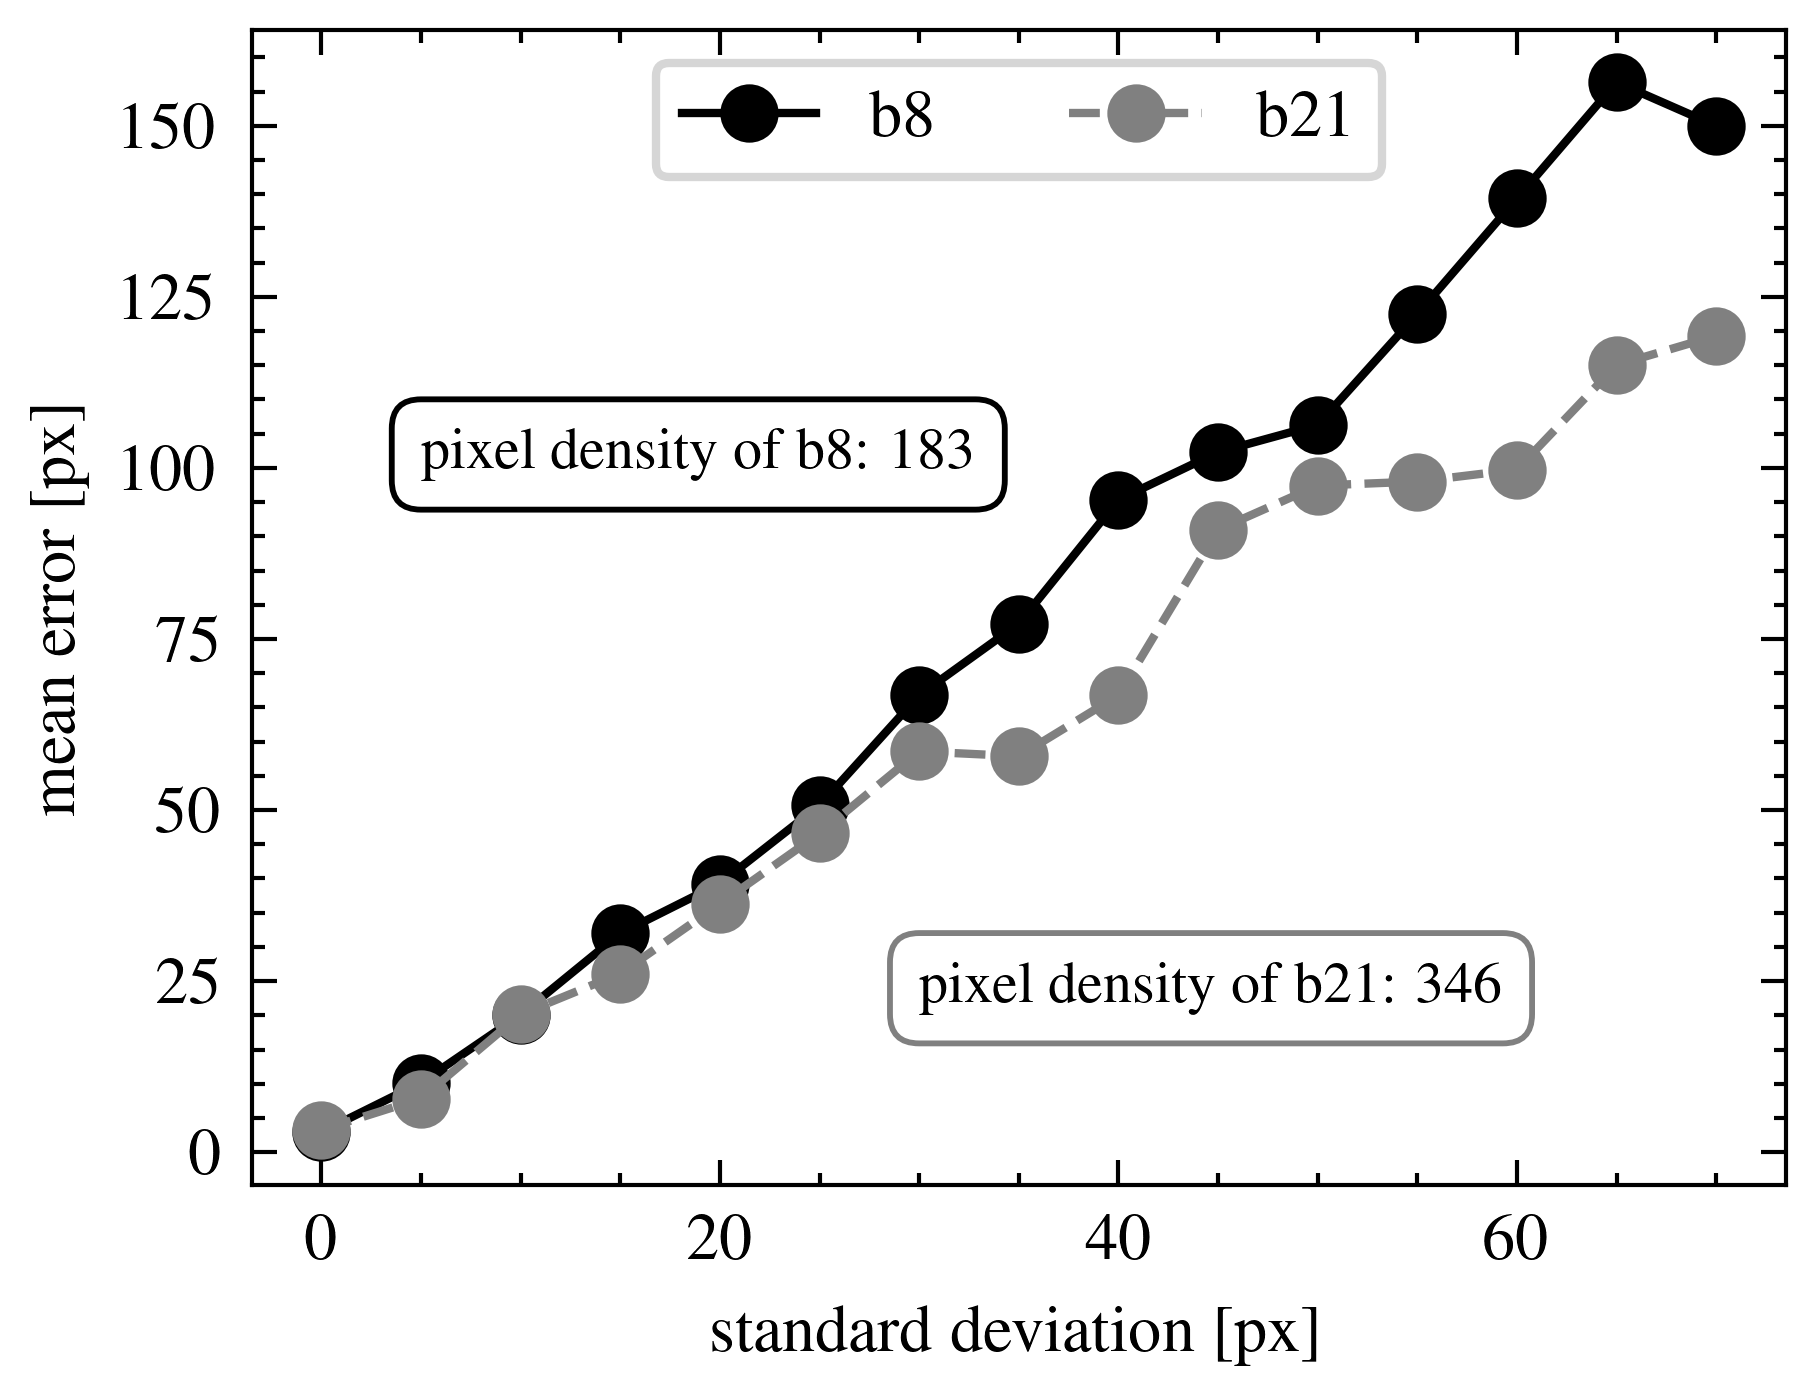
\includegraphics[width=0.40\textwidth]{figures/pixel_density_0026.png}
        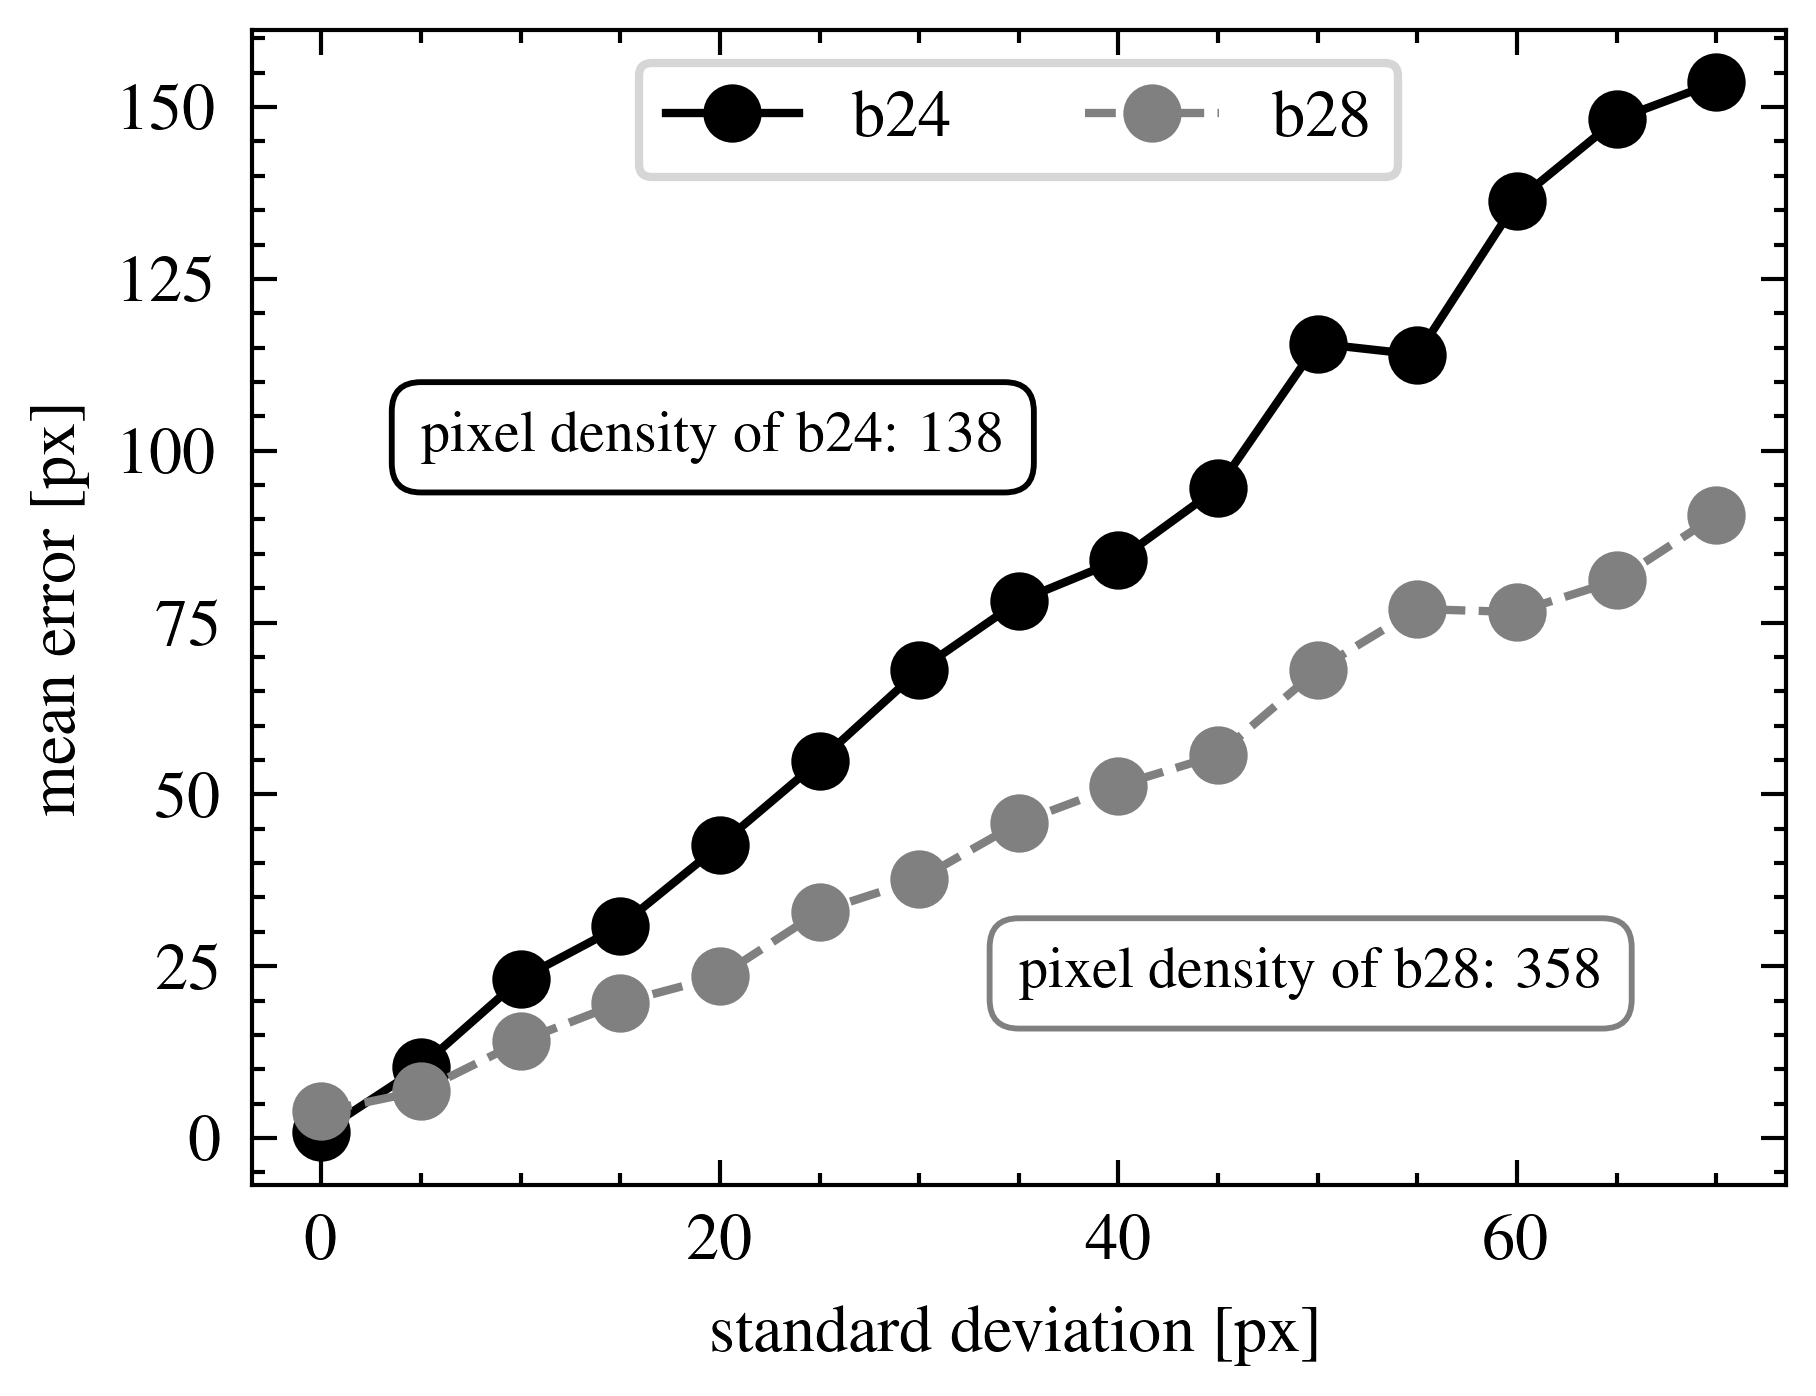
\includegraphics[width=0.40\textwidth]{figures/pixel_density_0029.png}
	\caption{The error for two similar points with different pixel densities 
		while increasing the random Gaussian noise around the reference 
		points, simulating measuring errors.}
	\label{fig:density}
\end{figure}

\subsection{Robustness}
We assess the robustness of our approach by considering two scenarios. 
First, we add random Gaussian noise to our reference point pairs and 
analyze the effect. Next, we introduce significant noise to specific 
reference point pairs to simulate outliers and re-evaluate the impact.

\subsubsection{Random Gaussian Noise}
To introduce further measurement errors to our experimental setup, we  
add random Gaussian noise with a mean of zero to the reference points in 
both the top- and perspective view. Again, we will increase the standard 
deviation by five pixels up to 70. We use every reference point available 
within IMG\_01 to calculate the homography, and determine the error with 
the validation points. We repeat this process 100 times for every 
standard deviation. Figure \ref{fig:random_noise}
shows the results. The error increases rapidly as the noise grows. Yet,
some minor measurement errors are acceptable.

\begin{figure}
	\begin{center}
		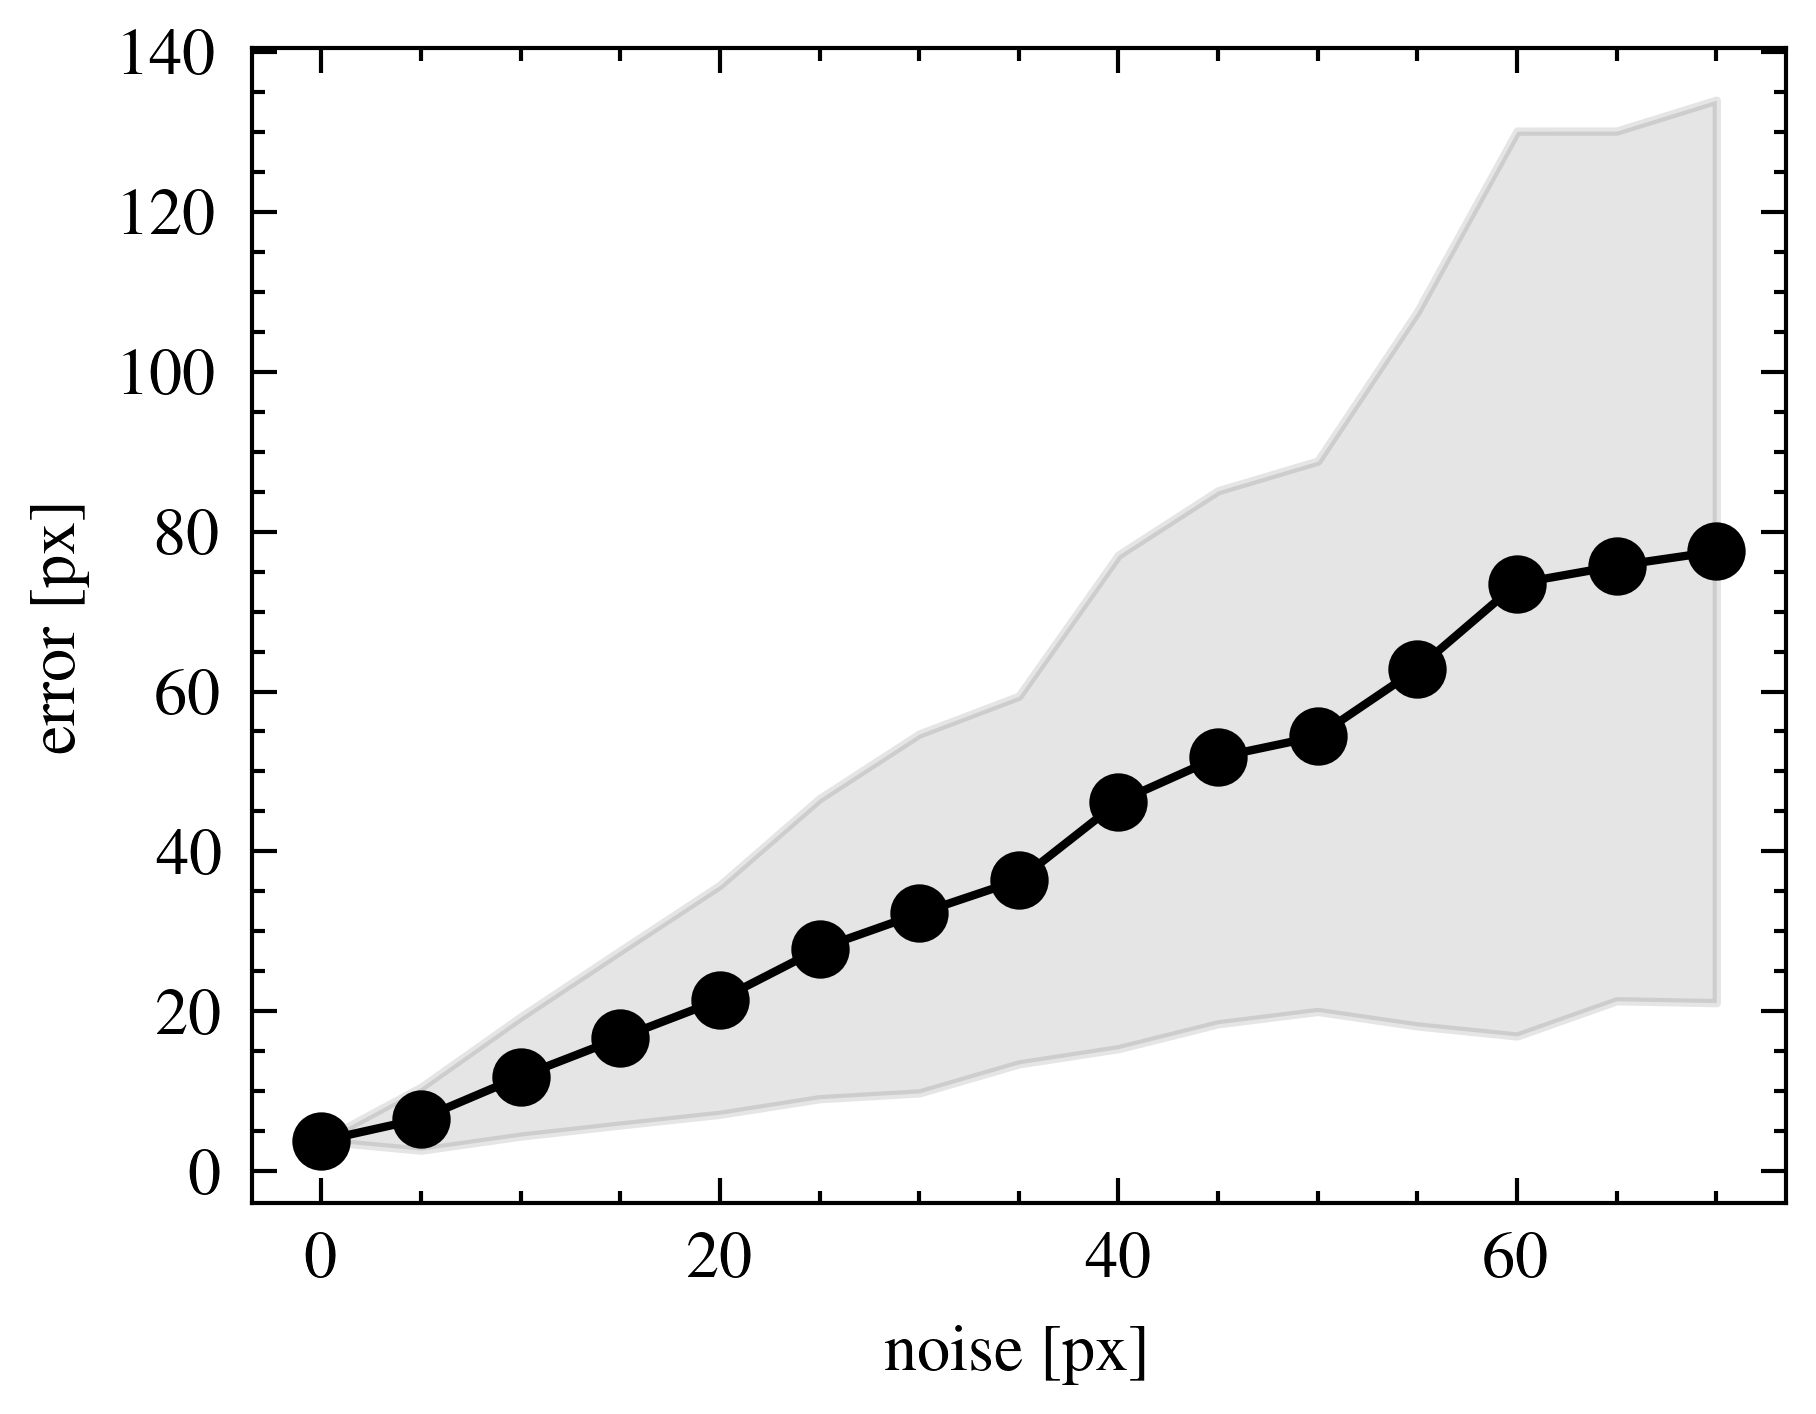
\includegraphics[width=0.40\textwidth]{figures/noise_results.png}
	\end{center}
	\caption{The error curve while applying additional noise to the 
	reference points.}
	\label{fig:random_noise}
\end{figure}

\subsubsection{Outliers} 
Additionally, we assess the impact of outliers by introducing significant 
noise to specific reference point pairs and moving them randomly. Previously, 
we used the least-squares optimization. 
However, least squares is not well-suited for handling outliers, making 
RANSAC the preferable choice. Figure \ref{fig:outliers} shows the setup, 
resulting in an error of $6.50$ cm for RANSAC and $543.40$ cm for 
least squares.

\begin{figure}
	\begin{center}
		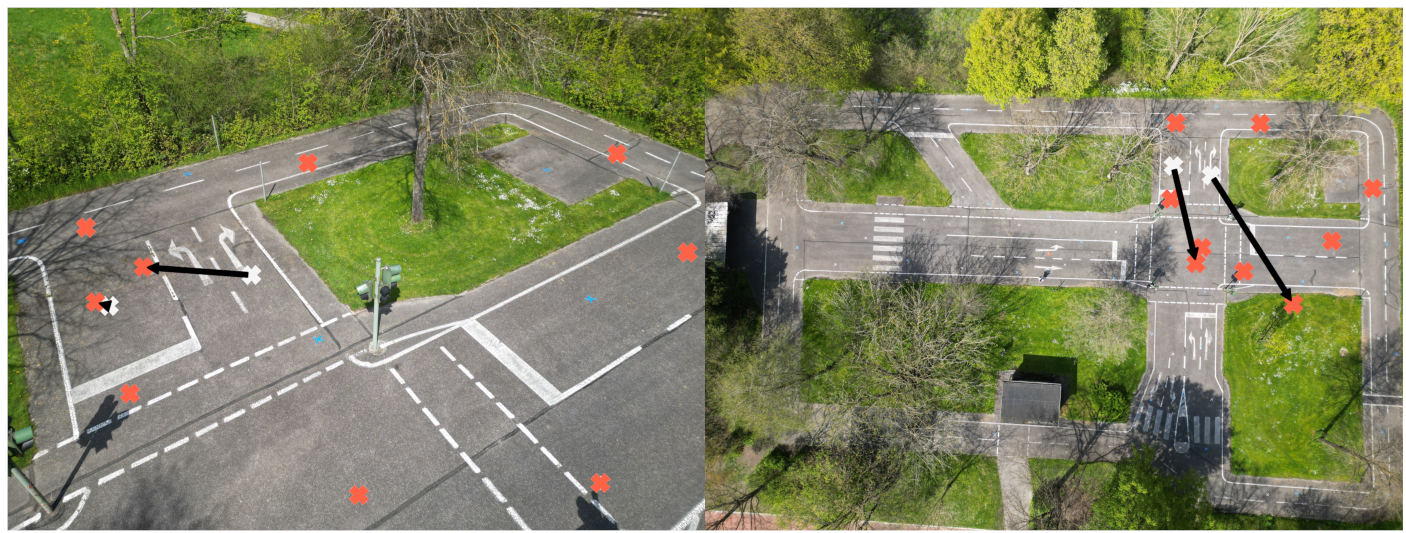
\includegraphics[width=0.45\textwidth]{figures/setup_outlier.png}
	\end{center}
	\caption{Producing two outliers for the reference points.}\label{fig:outliers}
\end{figure}

\subsection{Perspective}
Perspective influences our experimental results. The lower the camera and its 
pitch, the greater the distance imbalance among our 
validation points. Close validation points have high pixel densities, while 
distant validation points have low pixel densities. This imbalance increases 
the variance in errors. In this section, we have already examined how 
lower pixel densities can lead to higher errors.

Table \ref{tab:results_overall} shows that images with low 
perspectives (such as IMG\_06 or IMG\_08) have significantly 
higher errors than others. However, perspective is only one 
factor\textemdash collinearity and suboptimal reference point compositions 
also contribute to the errors. Nonetheless, perspective magnifies 
these effects and generally introduces more measurement errors.

